\chapter{Supervised learning}
We limit our focus to supervised and later on unsupervised learning if not specified otherwise, reinforcement learning will be treated later on.
\todo{Solve problem with bold greek letters}
\section{More formal introduction into the idea of Machine Learning}
\subsection{Problem set-up and recipe}
\label{subsec:recipeML}
Problems in ML typically involve inference about complex systems where we do not know the exact form of the mathematical model that describes the system. It is therefore not uncommon to have multiple candidate models that need to be compared.
\subsubsection{Ingredients}
Many problems in ML and data science start with the same ingredients. The first ingredient is the dataset $\mD=(\mX,\mathbf{y})$ where $\mX$ is a matrix of independent variables and $\mathbf{y}$ is a vector of dependent variables. The second is the model $f(\mx;\mt)$, which is a function $f:\mx \rightarrow y$ of the \emph{parameters} $\mt$. That is, $f$ is a function used to predict an output from a vector of input variables. 
\marginpar{Using polynomial models (i.e. polynomials of different order) in polynomial regressions, we can think of each term in the polynomial as a ’feature’ (i.e. a,b are features for $f_1(x)=a x^2+bx$) in our model, then increasing the order of the polynomial we fit increases the number of features.}
\begin{mybox}{Model class}
	To make predictions, we will consider a family of functions $f_{\alpha}(x,\mt_\alpha)$ that depend on some parameters $\mt_\alpha$. These functions represent the \emph{model class} that we are using to model the data and make predictions. Note that we choose the model class without knowing the function $f(x)$. The $f_\alpha(x;\mt_\alpha)$ encode the \emph{features} we choose to represent the data. Different models (e.g. $\alpha=1,2,3$) can contain different number of parameters, then the models have different \emph{model complexity}.
\end{mybox}
The final ingredient is the \emph{cost function} $\mC(\my,f(\mX;\mt))$ that allow us to judge how well the model performs on the observations $\my$. The model is fit by finding the value of $\mt$ that minimizes the cost function. For example, one commonly used cost function is the squared error. Minimizing the squared error cost function is known as the method of least squares, and is typically appropriate for experiments with Gaussian measurement errors.
\subsubsection{Recipe}
\begin{enumerate} 
\item The \emph{first step} in the analysis is to \emph{randomly} divide the dataset $\mD$ into two mutually exclusive groups $\mD_{train}$ and $\mD_{test}$ called the training and test sets. The fact that this must be the first step should be heavily emphasized - performing some analysis (such as using the data to select important variables) before partitioning the data is a common pitfall that can lead to incorrect conclusions. Typically, the majority of the data are partitioned into the training set (e.g. $90\%$) with the remainder going into the test set. 
\begin{mybox}{Cross evaluation}
	Therefore, to learn the parameters $\mt_\alpha$, we will train our models on a \emph{training dataset} and then test the effectiveness of the model on a \textbf{different} dataset, the \emph{test dataset}.
\end{mybox}
\item The model is fit by minimizing the cost function using only the data in the training set $\hat{\mt}= \arg \min_{θ}\{\mC(\my_{train}, f(\mX_{train};\mt) )\}$.
\item Finally, the performance of the model is evaluated by computing the cost function using the test set $\mC(\my_{test},f(\mX_{test};\hat{\mt}))$. 
\end{enumerate}
\subsection{Performance evaluation}
\label{subsec:performanceeval}
\subsubsection{Ingredients for performance evaluation}
\begin{mybox}{Measure for evaluating performance}
	The value of the cost function for the best fit model on the training set is called the \emph{in-sample error}
	\be 
	\label{eq:errorInsample}
	E_{in}=\mC(\my_{train},f(\mX_{train};\mt))
	\ee 
	and the value of the cost function on the test set is called the \emph{out-of-sample error}
	\be 
	\label{eq:errorOutsample}
	E_{out}= \mC(\my_{test},f(\mX_{test};\mt)).
	\ee 
	One of the most important observations we can make is that \textbf{the out-of-sample error is almost always greater than the in-sample error}
	\be 
	\label{eq:errorComparison}
	E_{out} \geq E_{in}.
	\ee 
	Comparison of candidate models is usually done by using $E_{out}$. The model that minimizes this out-of-sample error is chosen as the best model (i.e. model selection).
\end{mybox}
Note that once we select the best model on the basis of its performance on $E_{out}$, the real-world performance of the winning model should be expected to be slightly worse because the test data was now used in the fitting procedure.\\
Splitting the data into mutually exclusive training and test sets provides an unbiased estimate for the predictive performance of the model - this is known as \emph{cross-validation}.
\begin{mybox}{Pitfalls for performance evaluation}
	\label{subsubsec:performanceevalCurseDimensionality}
	It may be at first surprising that the model that has the lowest out-of-sample error $E_{out}$ usually \emph{does not} have the lowest in-sample Error $E_{in}$. Therefore, if our goal is to obtain a model that is useful for prediction, we may not want to choose the model that provides the best explanation for the current observations. At first glance, the observation that the model providing the best explanation for the current dataset probably will not provide the best explanation for future datasets is very counter-intuitive. \\
Moreover, the discrepancy between $E_{in}$ and $E_{ou}$ becomes more and more important, as the complexity of our data, and the models we use to make predictions, grows. As the number of parameters in the model increases, we are forced to work in high-dimensional spaces. The ’curse of dimensionality’ ensures that many phenomena that are absent or rare in low-dimensional spaces become generic.
\end{mybox}
A comment on the difference between the in-and out-of-sample errors:\\
There is a fundamental difference between minimizing the in-sample error and minimizing the out-of-sample error. The underlying reason for this is that the training data may not be representative of the full data distribution. From a Bayesian point of view, as David MacKay likes to repeat: \emph{We can't make predictions without making assumptions}. Thus, it is sensible to introduce priors that reflect the fact that we are likely to be undersampled (especially in high dimensions).
\subsubsection{Another mathematical measure for performance evaluation}
\begin{mybox}{$R^2$ coefficient of determination}
	 The model performance (in-sample and out-of-sample) can be evaluated using the so-called \emph{coefficient of determination}, which is given by:
		\be
	\label{eq:errorR2}
	R^2=1-\frac{\sum_{i=1}^n \abs{y^{true}_i - y^{pred}_i}^2}{\sum_{i=1}^n \abs{y^{true}_i- \frac{1}{n} \sum_{i=1}^n y^{pred}_i}^2}.
	\ee 
Optimal performance is $R^2=1$, but it can also be negative. A constant model that always predicts the expected value of $y, ⟨y^{true}⟩,$ disregarding the input features, would get a $R^2$ score of $0$.
\end{mybox}
















\subsubsection{How to effectively do the performance evaluation}
It turns out that for complicated models studied in ML, predicting and fitting are very different things.\\
	Models that give the best fit to existing data do not necessarily make the best predictions even for simple tasks. At small sample sizes, noise can create fluctuations in the data that look like genuine patterns. Simple models (like a linear function) cannot represent complicated patterns in the data, so they are forced to ignore the fluctuations and to focus on the larger trends. 
\begin{mybox}{Overfitting}
	\label{subsubsec:overfitting}
Complex models with many parameters can capture both the global trends and noise-generated patterns at the same time. In this case, the model can be tricked into thinking that the noise encodes real information. This problem is called \emph{overfitting} and leads to a steep drop-off in predictive performance.\\
We can guard against overfitting in two ways:
\begin{enumerate}
	\item We can use less expensive models with fewer parameters, or
	\item we can collect more data so that the likelihood that the noise appears patterned decreases.
\end{enumerate}
The relative degree of overfitting: This information is contained in the difference in accuracy of our model on the training  and test datasets.
\end{mybox}
\begin{mybox}{Bias-Variance tradeoff}
	\label{subsubsec:biasvariancetradeoff}
	The \emph{bias-variance} tradeoff is used in our countermeasures against overfitting. What is it ?\\When the amount of training data is limited, one can often get better predictive power performance by using a less expressive model rather than the more complex model. The simpler model has more ’bias’ but is less dependent on the particular realization of the training dataset, i.e. less ’variance’. Therefore, even though the correct model is guaranteed to have better predictive performance for an infinite amount of training data (less bias), the training errors stemming from finite-size sampling (variance) can cause simpler models to outperform the more complex model when sampling is limited.
\end{mybox}
The bias-variance tradeoff is one of the key concepts in ML and therefore discussed quantitatively in more detail in \ref{subsubsec:biasvariancetradeoff} and qualitatively in \ref{subsubsec:biasvarianceMathematicaloneClassifier}.\\
These two concepts are now discussed in more detail, for that we introduce another quantity and then look explicitly at the components of our theory causing problems for different complexity regimes.
\begin{mybox}{Bias}
	The bias represents the best our model could do if we had an infinite amount of training data to beat down sampling noise. The bias is a property of the kind of functions, or model class, we are using to approximate $f(x)$. In general, the more complex the model class we use, the smaller the bias. However, we do not generally have an infinite amount of data. For this reason, to get best predictive power it is better to minimize the out-of-sample error, $E_{out}$, rather than the bias. 
\end{mybox}\footnote{This stems from the the law of large number. This is a theorem that describes the result of performing the same experiment a large number of times. According to the law, the average of the results obtained from a large number of trials should be close to the expected value and will tend to become closer to the expected value as more trials are performed}
How can we get a better idea of what is the true object to minimize to get bets results ? \\
The Bias-Variance tradeoff is implicitly encoded in the in-and out-of-sample errors. We will therefore draw from statistical learning theory in the following to get a better understanding of what it is we ought to be doing to achieve best practices.\\
\subsubsection{Where do the insights about how to do best practices come from ?}
The out-of-sample error will decrease with the number of data points. As the number of data points gets large, the sampling noise decreases and the training data set becomes more representative of the true distribution from which the data is drawn. For this reason, in the infinite data limit, the in-sample and out-of-sample error must approach the same value, which is called the ’bias’ of our model.

\begin{figure}[h!]
	\centering
	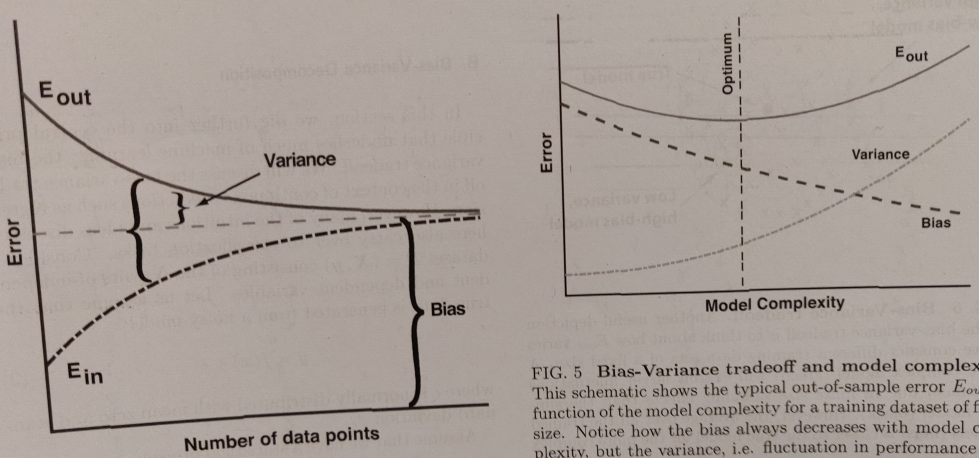
\includegraphics[width=0.7\linewidth]{gfx/InOutError.png}
	\caption{}
	\label{fig:errorbehaviour}
\end{figure}
Compare the behaviour of both errors with increasing number of data points, left graph of \ref{fig:errorbehaviour}, and the out-of-sample error with increasing model complexity, right graph of \ref{fig:errorbehaviour}. As for the left graph, we can look at the difference between the generalization ($E_{out}$) and training error ($E_{in}$), i.e. the big curly bracket representing $\abs{E_{in}-E_{out}}$. It measures how well our in-sample error reflects the out-of-sample error, and measures how much worse we would do on a new data set compared to our training data. For this reason, the difference between these errors is precisely the quantity that measures the difference between fitting and predicting. \emph{Models with a large difference between the in-sample and out-of-sample errors are said to \textbf{overfit} the data}. 
\begin{mybox}{}
	One of the lessons of statistical learning theory is that it is not enough to simply minimize the training error, because the out-of-sample error can still be large.
\end{mybox}
Considering the right graph, model  complexity is, in many cases, related to the number of parameters we are using to approximate the true function $f(x)$. If we consider a training dataset of a fixed size, $E_{out}$ will be a non-monotonic function of the model complexity, and is generally minimized for models with \emph{intermediate} complexity. The underlying reason for this is that, even though using a more complicated model always reduces the bias, at some point the model becomes too complex for the amount of training data and the generalization error becomes large due to high variance.
\begin{mybox}{}
Thus, to minimize $E_{out}$ and maximize our predictive power, it may be more suitable to use a more biased model with small variance than a less-biased model with large variance. This is is, again, the \emph{bias-variance} tradeoff we introduced above.
\end{mybox} 
Another way to understand this tradeoff is the following. Due to sampling noise from having finite size data sets, the learned models will differ for each choice of training sets. In general, more complex models need a larger amount of training data. For this reason, the fluctuations in the learned models (variance) will be much larger for the more complex model than the simpler model. However, if we consider the asymptotic performance as we increase the size of the training set (the bias), it is clear that the complex model will eventually perform better than the simpler model. Thus, depending on the amount of training data, it may \textbf{be more favourable to use a less complex, high-bias model to make predictions}.
























\section{Statistics}
Statistical modelling revolves around estimation or prediction.
\subsection{Difference between estimation and prediction}
Note first and foremost that techniques in ML tend to be more focused on prediction rather than estimation, which means that we will mostly treat prediction problems in this compendium. This is for example because an artificially intelligent agent needs to be able to recognize objects in its surroundings and predict the behaviour of its environment in order to make informed choices.\\
\subsubsection{Contrasting the two}
Estimation and prediction problems can be cast into a common conceptual framework. In both cases, we choose some observable quantity $\mx$ of the system we are studying (e.g. an interference pattern) that is related to some parameters $\mt$ (e.g. the speed of light) of a model $p(\mx|\mt)$ that describes the probability of observing $\mx$ given $\mt$.\\
Now we perform an experiment to obtain a dataset $\mX$ and use these data to fit the model. Typically,  ’fitting’ the model involves finding $\hat{\mt}$ that provides the best explanation for the data. In the case when ’fitting’ refers to the method of least squares, the estimated parameters maximize the probability of observing the data (i.e., $\hat{\mt}=\arg \max_{\mt}\{p(\mX|\mt) \}$).\\
\begin{mybox}{Estimation vs Prediction}
	\emph{Estimation problems} are concerned with the accuracy of $\hat{\mt}$, whereas \emph{prediction problems} are concerned with the ability of the model to predict new observations (i.e., the accuracy of $p(\mx|\hat{\mt})$. Although the goals of estimation and prediction are related, they often lead to different approaches.
\end{mybox}


\subsection{Mathematical motivation to presented key ideas}
We begin with an unknown function
$y = f (x)$ and fix a \emph{hypothesis set} $\mH$ consisting of all functions we are willing to consider, defined also on the domain of $f$ . This set may be uncountably infinite (e.g. if
there are real-valued parameters to fit). The choice of
which functions to include in $\mH$ usually depends on our
intuition about the problem of interest. The function
$f (x)$ produces a set of pairs $(x_i , y_i ), i = 1 . . . N$ , which
serve as the observable data. Our goal is to select a function from the hypothesis set $h \in \mH$ that approximates
$f (x)$ as best as possible, namely, we would like to find
$h \in \mH$ such that $h \approx f$ in some strict mathematical
sense which we specify below. 
\begin{mybox}{}
If this is possible, we say
that we \emph{learned} $f (x)$. 
\end{mybox}
But if the function $f (x)$ can, in
principle, take any value on \emph{unobserved inputs}, how is it
possible to learn in any meaningful sense ?\\
The answer is that learning is possible in the restricted
sense that the fitted model will probably perform approximately as well on new data as it did on the training data.
How can we evaluate the performance of our model then ?\\
As discussed in \ref{subsec:performanceeval}, once an appropriate error function $E$ is chosen for the
problem under consideration (e.g. sum of squared errors
in linear regression), we can define the in-and out-of-sample error to then minimize the out-of-sample error, with the variance-bias tradeoff in mind, to achieve robust predictions.
\subsubsection{Bias-Variance Decomposition for one Classifier}
\label{subsubsec:biasvarianceMathematicaloneClassifier}
Here we give a mathematical motivation to the bias-variance tradeoff discussed in \ref{subsubsec:biasvariancetradeoff}.\\
Consider a
dataset $\mD = (\mx, \mathbf{y})$ consisting of the $N$ pairs of independent and dependent variables. Let us assume that the
true data is generated from a noisy model
\be 
y = f (x) + \epsilon
\ee 
where $\epsilon$ is normally distributed with mean zero and standard deviation $\sigma_\epsilon$, i.e. the ’noise’.
Assume that we have a statistical procedure (e.g. least-
squares regression) for forming a predictor $f (\mx; \hat{\mathbf{θ}})$ that
gives the prediction of our model for a new data point $\mx$.
This estimator is chosen by minimizing a cost function
which we take to be the squared error
\be 
\label{eq:statCostFct}
\mC(\mathbf{y}, f(\mx; \mathbf{θ})) = \sum_i (y_i - f(x_i; \mathbf{θ}))^2.
\ee 
Therefore, the estimates for the parameters
\be 
\hat{\mathbf{θ}} =\arg \min_{θ} \mC(\mathbf{y}, f(\mx;\mathbf{θ}) )
\ee 
are a function of the dataset, $\mD$. We would obtain a
different error $\mC( \mathbf{y}_j , f (\mx_j ; \hat{\mathbf{θ}}_{\mD_j}))$ for each dataset $\mD_j =
(\mathbf{y}_j , \mx_j )$ in a universe of possible datasets obtained by
drawing $N$ samples from the true data distribution. We
denote an expectation value over all of these datasets as
$\mathbb{E}_{\mD}$.


\begin{mybox}{Errors}
	Combining these expressions,
	we see that the expected \emph{out-of-sample error}
	\be 
	 E_{out} := \mathbb{E}_{\mD,\epsilon}[\mC(\mathbf{y}, f (\mx; \hat{\mathbf{θ}}_{\mD} ))],
	\ee 
	 can be decomposed as
	 \be 
	E_{out} = \text{Bias}^2 + \text{Var} + \text{Noise},
	\ee
	with
	\begin{align*}
	\text{Noise}&=\sum_i \sigma^2_\epsilon,\; \text{Var}=\sum_i \mathbb{E}_{\mD}[(f (\mx_i ; \hat{\mathbf{θ}}_{\mD} ) − \mathbb{E}_{\mD}[f (\mx_i ; \hat{\mathbf{{θ}}}_{\mD})])^2 ],\\
	\text{Bias}^2&=\sum_i (f (\mx_i ) − \mathbb{E}_{\mD}[f ((\mx_i ;\hat{(\mathbf{θ}}_{\mD} )])^2.
	\end{align*}
	The variance measures how much our estimator fluctuates due
	to finite-sample effects and the bias measures the deviation of the expectation value of
	our estimator (i.e. the asymptotic value of our estimator
	in the infinite data limit) from the true value.
\end{mybox}
This gives us a mathematical tradeoff of the concepts discussed in \ref{subsec:performanceeval} and in particular in \ref{fig:errorbehaviour}.
\begin{mybox}{Bias-variance trade-off}
	The bias-variance tradeoff summarizes the fundamental tension in machine learning, particularly supervised
	learning, between the complexity of a model and the
	amount of training data needed to train it. Since data
	is often limited, in practice it is often useful to use a
	less-complex model with higher bias – a model whose
	asymptotic performance is worse than another model –
	because it is easier to train and less sensitive to sampling
	noise arising from having a finite-sized training dataset
	(smaller variance).
\end{mybox}
\subsubsection{Bias-Variance Decomposition for Ensembles}
\label{subsubsec:biasvarianceMathematicalEnsemble}
We will discuss the bias-variance tradeoff in the context of continuous predictions such as regression \ref{sec:linearRegression}. However, many of the intuitions and ideas discussed here also carry over to classification tasks, cf. \ref{sec:logisticRegression}. Consider a data set consisting of data $\mX_{\mL}=\{(y_j,\mx_j),j=1\dots n \}$ as above. Assume that we have a statistical procedure (e.g. OLS \ref{eq:lregOLS})) for forming a predictor $\hat{g}_{\mL}(\mx)$ that gives the prediction of our model for a new data point $\mx$ given that we trained the model using a dataset $\mL$. We will now, however, consider an ensemble of estimators $\{\hat{g}_{\mL}(\mx_i)\}$. Given a dataset $\mX_{\mL}$ and hyper-parameters $\mt$ that parametrize members of our ensemble, we will consider a procedure that deterministically generates a model $\hat{g}_{\mL}(\mx_i,\mt)$ given $\mX_{\mL}$ and $\mt$. We assume that the $\mt$ includes some random parameters that introduce stochasticity into our ensemble (e.g. an initial condition for stochastic gradient descent or a random subset of features or data points used for training.) Concretely, with a given dataset $\mL$ one has a learning algorithm $\mA$ that generates a model $\mA(\mt,\mL)$ based on a deterministic procedure which introduced stochasticity through $\mt$ in its execution on dataset $\mL$. \\
We will be concerned with the expected prediction error of the \emph{aggregate ensemble predictor}
\be 
\label{eq:biasvarianceAggregateEnsemblePredictor}
\hat{g}^A_{\mL}(\mx_i,\{\mt\} ) = \frac{1}{M} \sum_{n=1}^M \hat{g}_{\mL}(\mx_i,\mt_m).
\ee 
For future reference, let us define the mean, variance and covariance (i.e. the connected correlation function in the language of physics), and the normalized correlation coefficient of a single randomized model $\hat{g}_{\mL}(\mx,\mt_m)$ as 
\begin{align}
	\label{eq:biasvarianceDefinitionsMoments}
	\mathbb{E}_{\mL,\mt_m}[\hat{g}_{\mL}(\mx,\mt_m)] &= \mu_{\mL,\mt_m}(\mx) \nonumber \\
	\mathbb{E}_{\mL,\mt_m}[\hat{g}_{\mL}(\mx,\mt_m)^2]- \mathbb{E}_{\mL,\mt_m}[\hat{g}_{\mL}(\mx,\mt)]^2 &= \sigma^2_{\mL,\mt_m}(\mx) \nonumber \\
	\mathbb{E}_{\mL,\mt_m}[\hat{g}_{\mL}(\mx,\mt_m) \hat{g}_{\mL}(\mx,\mt_{m^\prime})] -\mathbb{E}_{\mt}[\hat{g}_{\mL}(\mx,\mt_m) ]^2 &= C_{\mL,\mt_m,\mt_{m^\prime}} (\mx) \nonumber \\
	\rho(\mx) &= \frac{C_{\mL,\mt_m,\mt_{m^\prime}}(\mx) }{\sigma^2_{\mL,\mt}}.
\end{align}
Note that the expectation $\mathbb{E}_{\mL,\mt_m}[\cdot]$ is computed over the joint distribution of $\mL$ and $\mt_m$. Also by definition, we assume $m\neq m^\prime$.\\
Now, we can, as in \ref{subsubsec:biasvarianceMathematicaloneClassifier}, define the expected generalization (out-of-sample) error for the ensemble 
\begin{align}
\label{eq:biasvarianceGeneralizationErrorEnsemble}
\mathbb{E}_{\mL,\mt_m}[C(\mX,\hat{g}^A_{\mL}(\mx))] &= \mathbb{E}_{\mL,\epsilon,\mt} \left[ \sum_i (\my_i - \hat{g}^A_{\mL} (\mx_i,\{\mt\} ))^2\right]\nonumber \\
&= Bias^2(\mx_i) + Var(\mx_i)+ \sum_i \sigma^2_{\epsilon_i},
\end{align}
where one defines the bias of an aggregate predictor 
\be 
\label{eq:biasvarianceBiasEnesemble}
Bias^2(\mx) \equiv \left(f(\mx) - \mathbb{E}_{\mL,\mt}[\hat{g}^A_{\mL} (\mx,\{\mt\}) ]\right)^2
\ee 
and the variance as
\bse 
Var(\mx) = \mathbb{E}_{\mL,\mt}\left[ (\hat{g}^A_{\mL}(\mx,\{\mt\}) - \mathbb{E}_{\mL,\mt}[\hat{g}^A_{\mL}(\mx,\{\mt\})])^2 \right]. 
\ese 
So far the calculation for ensembles is almost identical to that of a single estimator, compare \ref{subsubsec:biasvarianceMathematicaloneClassifier}.
\begin{mybox}{Crux of Bias-Variance for Ensembles}
	However, since the aggregate estimator is a sum of estimators, its variance implicitly depends on the correlations between the individual estimators in the ensemble. One finds
	\be 
	\label{eq:biasvarianceVarianceEnsembleCrux}
	Var(\mx) = \rho(\mx) \sigma^2_{\mL,\mt} + \frac{1-\rho(\mx)}{M} \sigma^2_{\mL,\mt}.
	\ee 
	This \ref{eq:biasvarianceVarianceEnsembleCrux} is the key to understanding the power of random ensembles. Notice that by using large ensembles ($M\rightarrow \infty$), we can significantly reduce the variance, and for completely random ensembles where the models are uncorrelated ($\rho(\mx)=0$), maximally suppresses the variance !\\
	Thus, reducing the aggregate predictor beats down fluctuations due to finite-sample effects. They key, as \ref{eq:biasvarianceVarianceEnsembleCrux} indicates, is to \textbf{decorrelate the models as much as possible while still using a very large ensemble.}
\end{mybox}
\begin{mybox}{What does this do to the bias ?}
One can be worried that this comes at the expense of a very large bias. This turns out not to be the case. When models in the ensemble are completely random, the bias of the aggregate predictor is just the expected bias of a single model 
\bse 
Bias^2(\mx) = (f(\mx) - \mu_{\mL,\mt})^2.
\ese 
\textbf{Thus, for a random ensemble one can always add more models without increasing the bias.}
\end{mybox}

Therefore, the correlation between models that constitute the ensemble is the key property here. It is important for two reasons. First, holding the ensemble size fixed, averaging the predictions of correlated models reduces the variance less than averaging uncorrelated models. Second, in some cases, correlations between models within an ensemble can result in an \emph{increase} in bias, offsetting any potential reduction in variance gained from ensemble averaging.\\
This will be discussed in the context of bagging  \ref{subsubsec:ensemblesBagging}.










\subsection{Mathematical set-up of every problem ever}
As described quantitatively in \ref{subsec:recipeML}, every problem in ML can be designed via a recipe which is presented now qualitatively.\\
\subsubsection{Set-up of the notation}
Suppose we are given a dataset with $n$ samples $\mD = \{(y_i,\mx^{(i)} )\}^n_{i=1}$, where $\mx^{(i)}$ is the $i$-th observation vector while $y_i$ is its corresponding (scalar) response. We assume that every sample has $p$ \emph{features}, namely,
\bse 
\mx^{(i)} \in \mR^p.
\ese  
Let $f$ be the true function/model that generated these samples via
\bse 
y_i  = f(\mx^{(i)}, \mw_{true}) + \epsilon_i,
\ese 
where $\mw_{true}\in \mR^p$ is a \emph{parameter} vector and $\epsilon_i$ is some i.i.d. white noise with zero mean and finite variance. Conventionally, we cast all samples in an $n\times p$ matrix, the \emph{design matrix}
\bse 
\mX \in \mR^{n\times p}
\ese 
with the rows 
\bse 
\mX_{i,:} = \mx^{(i)} \in \mR^p,\quad i =1,\dots,n
\ese 
being \emph{observations} and the columns
\bse 
\mX_{:,j} \in \mR^n,\quad j=1,\dots,p 
\ese 
being measured \emph{features}(i.e. feature predictors).\\
Bear in mind that this function $f$ is never known to us explicitly, though in practice we usually presume its functional form.
\begin{example}
	For example, in \emph{linear regression}, we assume
	\bse 
	y_i = f(\mx^{(i)};\mw_{true}) + \epsilon_i= \mw^T_{true} \mx^{(i)} + \epsilon_i
	\ese 
	for some unknown but fixed $\mw_{true}\in \mR^p$.
\end{example}










\subsubsection{Set-up of the problem}
We want to find a function $g$ with parameters $\mw$ fit to the data $\mD$ that can best approximate $f$. This is done when we have found a $\hat{\mw}$ such that $g(\mx;\hat{\mw})$ yields our best estimate of $f$. Now we can use this $g$ to make predictions about the response $y_0$ for a new data point $\mx_0$.\\
Therefore:\\
Fitting a given set of samples $(y_i,\mx_i)$ means relating the independent variables $\mx_i$ to their responses $y_i$. The next step is to assume some \emph{models} that might explain the measurements and measuring their performance, i.e. finding the function $g$ such that
\bse 
y_i = g(\mx_i;\mw).
\ese 
We call $g(\mx^{(i)},\mw)$ the \emph{predictor}. Recall that the optimal choice of predictor depends on, among many other things, the functions used to fit the data and the underlying noise level.
We then try to minimize the errors made in explaing the given set of measurements based on our model $g$ by tuning the parameters $\mw$. To do so, we need to first define the error function (formally called the  \emph{loss function}) that characterizes the deviation of our prediction from the actual response




\subsubsection{On statistical language}
As described above, a ML or statistics problem is defined via a optimization (minimization) problem of an error function, the solution to this is given by some estimator
\be 
\hat{\mw}_{Problem} = \arg \min_{\mw \in \mR^p} \mC(\mX, g(\mw,\my)).
\ee 
The bias (or bias function) of an estimator is the difference between this estimator's expected value and the true value of the parameter being estimated.


\subsection{Language of optimization problems}
\subsubsection{Convexity}
Recall that a set $C\subset\mR^n$ is called \emph{convex} if any  $x,y\in C$  and  $t\in [0,1]$,
\bse 
tx + (1-t) y \in C.
\ese 

In other words, every line segments joining  $x,y$  lies entirely in  $C$ .

A function $f:\mR^n \rightarrow \mR$ is called \emph{convex} if its domain $\text{dom}(f)$  is a convex set and for any  $x,y\in \text{dom}(f)$  and $ t\in[0,1]$ ,
\bse 
f(tx+(1-t)y) \leq t f(x) + (1-t) f(y).
\ese 

In other words, the function lies below the line segment joining $ f(x)$  and $ f(y)$ . This function  $f$  is called \emph{strictly convex} if this inequality holds strictly for  $x \neq y$  and  $t \in (0,1)$ .
\begin{mybox}{}
Why is convexity important? \\
\textbf{For convex functions, any local minimizer is a global minimizer}. Algorithmically, this means that in the minimization (optimization) procedure, as long as we're "going down the hill" and agree to stop when we can't go any further, then we've hit the global minimum. In addition to this, there's a menagerie of beautiful theory regarding convex duality and optimality, which gives us a way of understanding the solutions even before solving the problem itself.
\end{mybox}


\section{Overview of Bayesian Inference}
\label{sec:bayes}
Bayesian inference provides a set of principles and procedures for learning from data and for describing uncertainty.
\subsection{Language}
\begin{mybox}{Likelihood function}
	The \emph{likelihood function} 
	\be
	\label{eq:bayesLikelihoodFct}
	p(\mX|\mt)
	\ee 
	describes the probability of observing a dataset $\mX$ for a given value of the unknown parameters $\mt$. It is a function of the parameters $\mt$ with the data $\mX$ held fixed. Furthermore, it is determined by the model and the measurement noise.
\end{mybox}
\begin{mybox}{Prior distribution}
	The \emph{prior distribution} $p(\mt)$ describes any knowledge that we have about the parameters before we collect the data.
\end{mybox}
\begin{mybox}{Priors}
	\label{subsec:priors}
	There are two general classes of priors: 
	\begin{enumerate}
		\item The \emph{uninformative prior}:\\
		We choose this one if we do not have any specialized knowledge about $\mt$ before we look at the data. 
		\item The \emph{informative prior}:\\
		If we have prior knowledge, we choose an informative prior that accurately reflects the knowledge that we have about $\mt$. This one is commonly employed in ML:
	\end{enumerate}
	There is another not so important prior, the \emph{hierarchical prior}. This describes the process of choosing a hyperparameter by defining a prior distribution for it (via an uninformative prior) and then averaging the posterior distribution over all choices of the hyperparameter.
\end{mybox}
Using an informative prior tends to decrease the variance of the posterior distribution while, potentially, increasing its bias. It is beneficial if the decrease in variance is larger than the increase in bias. In high-dimensional problems, it is reasonable to assume that many of the parameters will not be strongly relevant. Therefore, many of the parameters of the model will be zero or close to zero. We can express this belief using two commonly used priors.
\begin{mybox}{Two informative priors commonly employed}
	The \emph{Gaussian prior} is used to express the assumption that many of the parameters will be small 
	\be 
	\label{eq:bayesGaussianprior}
	p(\mt|\lambda) = \prod_j \sqrt{\frac{\lambda}{2 \pi}} e^{- \lambda \theta^2_j},
	\ee
	where $\lambda$ is a \emph{hyperparameter}. The \emph{Laplace prior} is used to express the assumption that many of the parameters will be zero
	\be 
	\label{eq:bayesLaplacianprior}
	p(\mt|\lambda) = \prod_j \frac{\lambda}{2} e^{-\lambda \abs{\theta_j}}.
	\ee 
	The hyperparameter can either be chosen via a hierarchical prior employing MCMC or  by simply finding a good value of $\lambda$ using an optimization procedure (see linear regression).
\end{mybox}
Indeed, a Gaussian prior is the \emph{conjugate prior} that gives a Gaussian posterior. For a given likelihood, conjugacy guarantees the preservation of prior distribution at the posterior level.
\begin{example}
	For example, for a Gaussian (Geometric) likelihood with a Gaussian (Beta) prior, the posterior distribution is still a Gaussian (Beta) distribution.
\end{example}
\begin{mybox}{hyperparameters}
	A \emph{hyperparameter} or \emph{nuisance variable} is a parameter whose value is set before the learning process begins. By contrast, the values of other \emph{parameters} are derived via training.
\end{mybox}

\subsubsection{Connecting statistics and bayesian framework}
To connect a statistical model to the Bayesian framework, we often write the model as
\be 
\label{eq:bayesianFreqConnectionModel}
p(y|\mx,\mt) = \mathcal{N}(y|\mu(\mx),\sigma^2(\mx)).
\ee 
In other words, our model is defined by a conditional probability that depends not only on data $\mx$ but on some model parameters $\mt$.
\begin{example}
	For example, if the mean is a linear function of $\mx$ given by $\mu = \mx^T \mw$, and the variance is fixed $\sigma^2(\mx) = \sigma^2$, then $\mt=(\mw,\sigma^2)$.
\end{example}











\subsection{Calculations}
\begin{mybox}{Bayes' rule}
	The \emph{posterior distribution} $p(\mt|\mX)$ describes our knowledge about the unknown parameter $\mt$ after observing the data $\mX$. It is given via Bayes' rule
	\be 
	\label{eq:bayesrule}
	p(\mt | \mX) = \frac{p(\mX|\mt) p(\mt) }{\int \md \mt^\prime p(\mX | \mt^\prime) p(\mt^\prime)}.
	\ee
\end{mybox}
The denominator is difficult in practice such that one normally uses Markov Chain Monte Carlo (MCMC) to draw random samples from $p(\mt|\mX)$.
\subsection{Estimation}
\subsubsection{Maximum Likelihood estimation}
\label{subsubsec:bayesEstMLE}
In statistics, many problems rely on estimation of some parameters of interest.
\begin{example}
	For example, suppose we are given the height data of $20$ junior students from a regional high school, but what we are interested in is the average height of all high school juniors in the whole country. It is conceivable that the data we are given are not representative of the student population as a whole.
\end{example}
It is therefore necessary to devise a systematic way to perform reliable estimation. Here we present the \emph{maximum likelihood estimation} (MLE), and show that MLE for $\mt$ is the one that minimizes the mean squared error (MSE) used in \ref{eq:lregOLS}.
\begin{mybox}{MLE}
	Many common statistical procedures such as least-square fitting can be cast as MLE. In MLE, one chooses the parameters $\hat{\mt}$ that maximizes the likelihood (or equivalently the log-likelihood since log is a monotonic function) of the observed data $\mX$ (or equivalently $\mD$):
	\be 
	\label{eq:bayesMLE}
	\hat{\mt}= \arg \max_{\mt} \log p(\mX |\mt).
	\ee 
	In MLE we therefore choose the parameters that maximize the probability of seeing the observed data given our generative model.
\end{mybox}
Using the assumption that samples are i.i.d., we can write the \emph{log-likelihood} as 
\be 
\label{eq:bayesLogLikelihood}
l(\mt) \equiv \log p(\mD|\mt) = \sum_{i=1}^n \log p(y_i|\mx^{(i)},\mt).
\ee 
Note that the conditional dependence of the response variable $y_i$ on the independent variable $\mx^{(i)}$ in the likelihood function is made explicit since, in most applications, the observed value of data, $y_i$, is predicted based on $\mx^{(i)}$ using a model that is assumed to be a probability distribution that depends on unknown parameters $\mt$. This distribution, when endowed with $\mt$, can, as we hope, potentially explain our prediction on $y_i$. By definition, such distribution is the likelihood function \ref{eq:bayesLikelihoodFct}. We stress that this notation does \emph{not} imply $\mx^{(i)}$ is unknown, it is still part of the observed data!
\begin{mybox}{Error function}
The negative of the log-likelihood gives us the error function
\be 
\label{eq:bayesErrorFct}
E(\mt)=-l(\mt).
\ee 
\end{mybox}
\subsubsection{Maximum-a-Posteriori estimation}
\ref{eq:bayesMLE} provides the tools for computing the posterior distribution $p(\mt|\mX)$, which uses probability as a framework for expressing our knowledge about the parameters $\mt$. In most cases, however, we need to summarize our knowledge and pick a single ’best’ value for the parameters. In principle, the specific value of the parameters should be chosen to maximize a utility function. In practice, however, we usually use on of two choices:
\begin{enumerate}
	\item The posterior mean, or  \emph{Bayes estimate}
	\be 
	\label{eq:bayesBayesEstimate}
	\expval{\mt} = \int \md \mt \mt \;p(\mt |\mX),
	\ee 
	or
	\item the posterior mode, also called the \emph{maximum-a-posteriori} (MAP) estimate
	\be 
	\label{eq:bayesMAPestimate}
	\hat{\mt}_{MAP} = \arg \max_{\mt} p(\mt |\mX).
	\ee 
	This estimate gives the parameters at which the posterior probability distribution is peaked
\end{enumerate}
While the Bayes estimate minimizes the mean-squared error, MAP estimate is often used instead because it is easier to compute.
\subsubsection{Out-of-Bag estimators}
\label{subsubsec:bayesOOBestimators}
For ensemble methods, especially random forest \ref{subsec:ensemblesRandomForest}, there exists another object for estimation, the \emph{out-of-bag (OOB) estimates}.
This is discussed in more detail in \ref{subsec:ensemblesRandomForest}.
\subsection{Bayesian view on regularization}
As discussed in \ref{subsec:performanceeval}, \emph{we can't make predictions without making assumptions}. Thus, it is sensible to introduce priors that reflect the fact that we are likely to be undersampled (especially in high dimensions).\\
We can supplement an error function with a regularizer that prevents overfitting. From a Bayesian point of view, the regularization can be thought of as a prior on parameters. Minimizing the combined in-sample error $+$ regularization terms is the same as the \emph{Maximum a posteriori probability} (MAP) estimate in Bayesian regression \ref{eq:bayesMAPestimate}. Note that in a true Bayesian approach, we should not use the mode of the posterior but the average over all possible choices of parameters weighted by their posterior probability. In practice, this is often not done (for computational and practical reasons).
\subsubsection{MAP estimator in the context of regularization}
Instead of maximizing the the log-likelihood \ref{eq:bayesLogLikelihood} to obtain a good estimator \ref{eq:bayesMLE},  let us maximize the log posterior $\log p(\mt|\mD)$, which we can get via Bayes' rule \ref{eq:bayesrule}. Then, the MAP estimator becomes 
\be 
\hat{\mt}_{MAP} \equiv \arg \max_{\mt} \log p(\mD|\mt) + \log p(\mt).
\ee 
A common choice for the prior $p(\mt)$ is the Gaussian distribution. Consider the Gaussian prior \ref{eq:bayesGaussianprior} with zero mean and variance $\tau^2$, namely
\bse 
p(\mw) =\prod_j \mathcal{N}(w_j|0,\tau^2).
\ese 
Then, we can recast the MAP estimator into
\begin{align}
	\label{eq:bayesMAPestimatorGaussianPrior}
	\hat{\mt}_{MAP} &= \arg \max_{\mt} \left[ -\frac{1}{2 \sigma^2} \sum_{i=1}^n (y_i-\mw^T \mx^{(i)} )^2 - \frac{1}{2 \tau^2 } \sum_{j=1}^n w^2_j\right]\nonumber \\
	&= \arg \max_{\mt} \left[- \frac{1}{2 \sigma^2} \norm{\mX \mw -\my }^2_2 - \frac{1}{2\tau^2} \norm{\mw}^2_2\right].
\end{align}
This is used later on to cast linear regression into bayesian language, \ref{subsec:lregBayesian}.




\section{Information theory}
\label{sec:info}



\subsection{Entropy as a measure of information}
\label{subsec:infoEntropy}
\subsubsection{Probabilities introduction}
To a set of measurement outcomes, or more general realizations of a random variable, one can associate symbols $\{x_1,\dots,x_N\}$ and probabilities $p(x_1),\dots,p(x_N)$ which are normalized $1=\sum_x p(x)$.\\
For two events $X$ and $Y$ with possible outcomes $\{x_m\}$ and $\{y_n\}$ one has a complete description in term of \emph{joint probabilities}
\be 
p(x_m,y_n),\quad 1=\sum_{x,y}p(x,y).
\ee 
If the two events are \emph{statistically independent} one has
\be 
p(x,y)=p(x)p(y),
\ee 
but that is of course not always the case. More general, the reduced (\emph{marginal}) probabilities for one event are
\be 
p(x)=\sum_y p(x,y),\quad p(y)=\sum_x p(x,y).
\ee 
Assume now that one has already learned the outcome $x_0$, then the new probability distribution for $y$ is
\be 
p(y_n |x_0) = \frac{p(x_0,y_n)}{\sum_k p(x_0,y_k)} = \frac{p(x_0,y_n)}{p(x_0)}
\ee 
which is the \emph{conditional probability}\footnote{Read: probability for $y_n$ under the condition that $x_0$ has been obtained.} One can write
\be 
p(x_m,y_n) = p(y_n |x_m) p(x_m)=p(x_m|y_n) p(y_n),
\ee 
which directly implies Baye's theorem \ref{eq:bayesrule}
\be 
p(x_m|y_n) = \frac{p(y_n|x_m) p(x_m)}{p(y_n)}.
\ee 
\subsubsection{Shannon's information entropy}
How much information can one learn from an outcome or event realization $x$ ? Or, in other words, how large is the information content $i(x)$ associated with the outcome $x$? Intuitively, the less likely the outcome, the higher the information content. Moreover, for independent events it is natural to take the information content additive,
\be 
i(p(x,y)) = i(p(x) p(y)) = i(p(x)) +i(p(y)).
\ee 
This directly leads to the logarithm, and the definition of the \emph{information content}
\be 
i(x)=i(p(x)) = -\ln p(x).
\ee 
In principle, one might add a (positive) prefactor here or, equivalently, take another base for the logarithm. Oftentimes $\log_2$ is used, but we work here with the natural logarithm in this section. For example, throwing an ideal coin corresponds to $p(x_1)=p(x_2)=\half$ and by learning the event outcome one learns an amount of information 
\be 
i=- \ln\half = \ln 2,
\ee 
corresponding to one bit of information. Note that a very unlikely event outcome with $p\rightarrow 0$ has formally infinite information content, $i\rightarrow \infty$. On the other side, a certain event outcome with unit probability, $p=1$, has no information content, $i=0$.
\begin{mybox}{Shannon's information entropy}
	Shannon's \emph{information entropy} associated to a discrete random variable or event $X$ is the expected amount of information content,
	\be
	\label{eq:infoShannon}
	H(X)=\expval{i(x)} = - \sum_x p(x) \ln p(x).
	\ee 
\end{mybox}



\subsection{Relative Entropy or Kullback-Leibler divergence}
\label{subsec:infoRelEntropy}
The KL divergence between two distributions $p(\mx)$ and $q(\mx)$ measures the dissimilarity between the two distributions and is given by
\be 
\label{eq:infoKLdivergence}
D_{KL}(q||p) = \text{Tr}_{\mx}q(\mx) \log \frac{q(\mx)}{p(\mx)},
\ee 
which is the expectation w.r.t. $q$ of the logarithmic difference between the two distributions $p$ and $q$ The trace denotes a sum over all possible configurations $\mx$. Two important properties of the KL-divergence are 
\begin{enumerate}
	\item Positivity: $D_{KL}(p||q)\geq 0$ with equality if and only if $p=q$, and
	\item the KL-divergence is not symmetric in its arguments $D_{KL}(p||q) \neq D_{KL} (q||p)$.
\end{enumerate}












\section{Mathematical tools}
\label{sec:math}
\subsection{Sampling methods}

\subsubsection{Empirical Bootstrapping}
\label{subsubsec:ensemblesBootstrapping}
Empirical bootstrapping is a method to enlarge a sparse dataset, we use it in bagging, cf. \ref{subsubsec:ensemblesBagging}.\\
Suppose we are given a finite set of $n$ data points $\mD=\{X_1,\dots,X_n\}$ as training samples and our job is to construct measures of confidence for our sample estimates (e.g. the confidence interval or mean-squared error of sample median estimator). To do so, one first samples $n$ points \textbf{with replacement} from $\mD$ to get a new set $\mD^{*(1)}=\{X^{*(1)}_1,\dots,X^{*(1)}_n\}$. called a \textbf{bootstrap sample}, which possibly contains repetitive elements. Then we repeat the same procedure to get in total $B$ such sets: 
\bse 
\mD^{*(1)},\dots, \mD^{*(B)}.
\ese 
The next step is to use these $B$ bootstrap sets to get the \textbf{bootstrap estimate} of the quantity of interest. For example, let $M^{*(k)}_n=$Median$(\mD^{*(k)})$ be the sample median of bootstrap data $\mD^{*(k)}$. Then we can construct the variance of the distribution of bootstrap medians as
\be 
\label{eq:ensemblesBootrapingVariance}
\hat{Var}_B(M_n)=\frac{1}{B-1} \sum_{k=1}^B \left[M^{*(k)}_n-\bar{M}^{*}_n\right]^2 = \sigma^2 \stackrel{n\rightarrow \infty}{\longrightarrow} \frac{1}{n}
\ee 
where 
\bse 
\bar{M}^{*}_n=\frac{1}{B} \sum_{k=1}^{B} M^{*(k)}_n
\ese 
is the mean of the median of all bootstrap samples.
\\
For $n\rightarrow\infty$, it was shown that the distribution of the bootstrap estimate will be a Gaussian centred around $\hat{M}_n(\mD)=$Median$(X_1,\dots,X_n)$ with standard deviation proportional to $1/\sqrt{n}$. This mean that the bootstrap distribution $\hat{M}^*_n-\hat{M}_n$ approximates fairly well the sampling distribution $\hat{M}_n-M$ from which we obtain the training data $\mD$. Note that $m$ is the median based on which the true distribution $\mD$ is generated. In other words, if we plot the histogram of $\{M^{*(k)}_n \}^B_{k=1}$, we will see that in the large $n$ limit it can be well fitted by a Gaussian which sharp peaks at $\hat{M}_n(\mD)$ and vanishing variance whose definition is given by \ref{eq:ensemblesBootrapingVariance}.

\begin{figure}[h!]
	\centering
	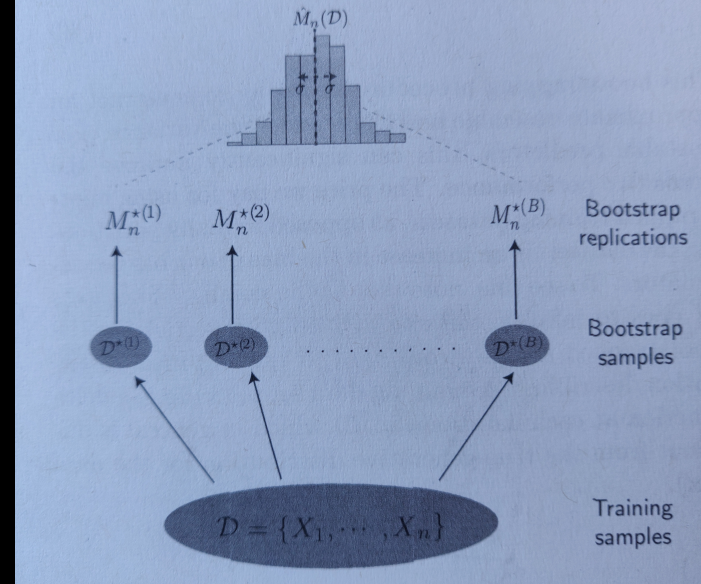
\includegraphics[width=0.7\linewidth]{gfx/Bootstrapping}
	\caption{}
	\label{fig:bootstrapping}
\end{figure}
Figure \ref{fig:bootstrapping} shows the procedure of empirical bootstrapping. 
\begin{mybox}{Bootstrapping - Summary}
	The goal is to assess the accuracy of a statistical quantity of interest, which in the main text is illustrated as the sample median $\hat{M}_m(\mD)$. We start from a given dataset $\mD$ and bootstrap $B$ size $n$ datasets $\mD^{*(1)},\dots,\mD^{*(B)}$ called the bootstrap samples. Then we compute the statistical quantity of interest on these bootstrap samples to get the median $M^{*(k)}_n$, for $k=1,\dots,B$. These are then used to evaluate the accuracy of $\hat{M}_n(\mD)$. It can be shown that in the $n\rightarrow\infty$ limit the distribution of $M^{*(k)}_n$ would be a Gaussian centred around $\hat{M}_n(\mD)$ with variance $\sigma^2$ defined by \ref{eq:ensemblesBootrapingVariance}.
\end{mybox}


\subsection{Algorithms}
\subsubsection{Decision Trees}
\label{subsubsec:ensemblesRFDecisionTree}
Decision trees are high-variance, weak classifiers that can be easily randomized, and as such, are ideally suited for ensemble-based methods.
They are employed for random forests, cf. \ref{subsec:ensemblesRandomForest}.\\
A decision tree uses a series of questions to hierarchically partition the the data. Each branch of the decision tree consists of a question that splits the data into smaller subsets with the leaves (end points) of the tree corresponding to the ultimate partitions of the data. When using decision trees for classification, the goal is to construct trees such that the partitions are informative about the class label. It is clear that more complex decision trees lead to finer partitions that give improved performance on the training set. However, this \textbf{generally leads to over-fitting}, limiting the out-of-sample performance. For this reason, in practice almost all decision trees use some form of regularization (e.g. maximum depth for the tree) to control complexity and reduce overfitting. Decision trees also have extremely high variance, and are often extremely sensitive to many details of the training data. This is not surprising since decision trees are learned by partitioning the training data. Therefore, \textbf{individual decision trees are weak classifiers.}\\
\\
However, these same properties make them ideal for incorporation in an ensemble method.\\
























